\section{Moderating Influences: Community Based Control on Misinformation Spread}
In this section, we examine the different misinformation ecosystems on Reddit. Largely in contrast to the self-organizing and porous communities that exist on Twitter, Reddit allows users to  establish their own self-contained communities. These communities known as subReddits have their own rules, communities norms, political preferences, as well as purposes. These subReddits module, control, and filter the content on Reddit platform. Behaviors in one subReddit that blocked or condemned in one subReddit can be widely celebrated in another subReddit. For example, one subReddit \texttt{r/conspiracy} that has over 1.7M (at time of writing in February 2022)  is dedicated to the discussion on conspiracy theories. Conspiracy Theories that are widely discussed in this subReddit are often ridiculed in other subReddit like \texttt{r/Qult\_Headquarters}.
\begin{figure*}
\begin{subfigure}{.48\textwidth}
  \centering
  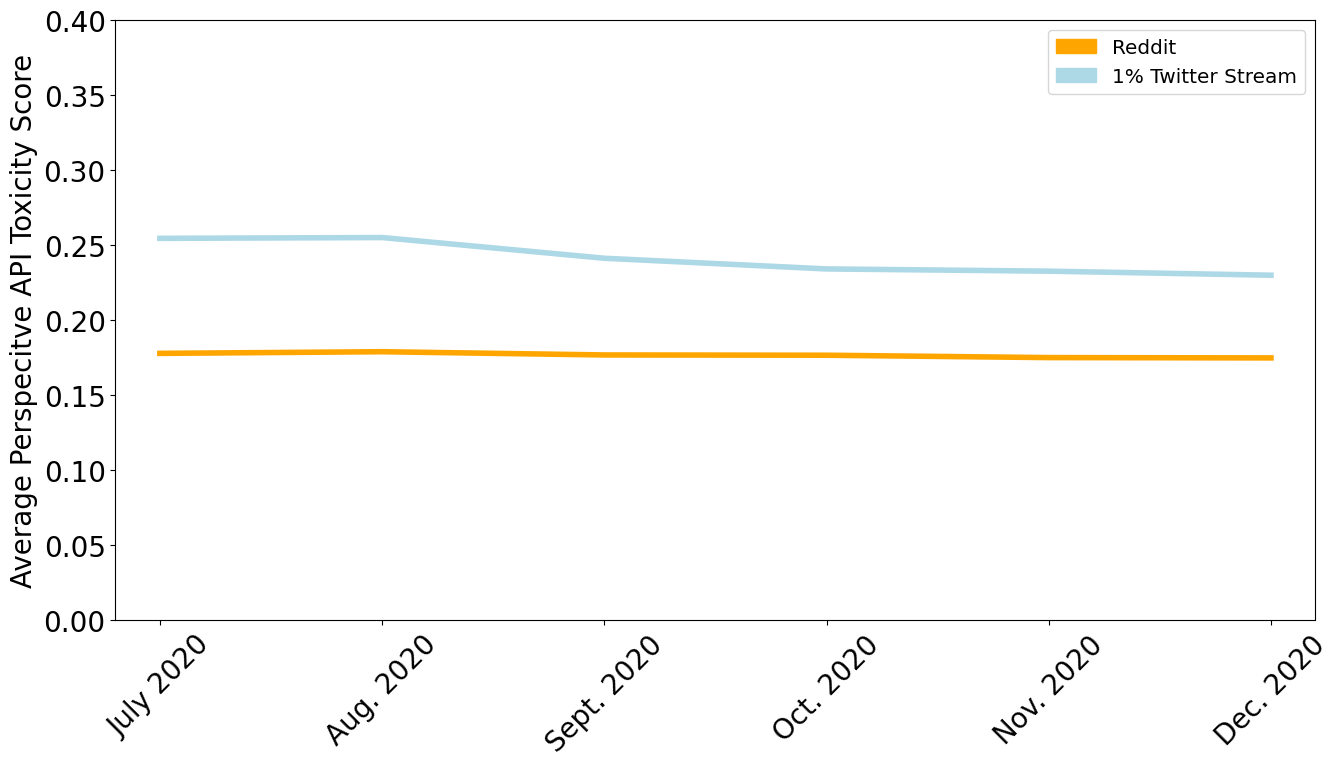
\includegraphics[width=1\linewidth]{figures/average-toxicity-end-2020.png}
\label{fig:cdf-subreddit-hyperlinks}
\end{subfigure}%
\begin{subfigure}{.48\textwidth}
  \centering
  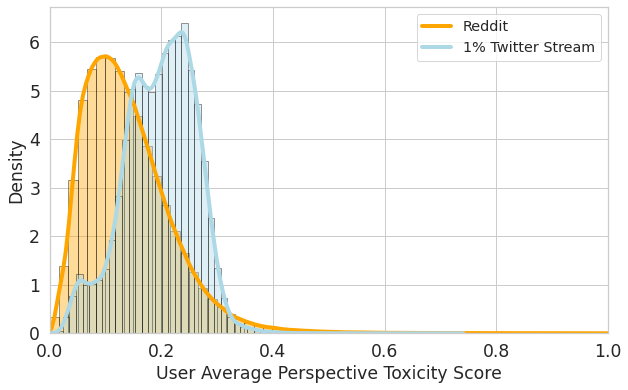
\includegraphics[width=1\linewidth]{figures/average-toxicity-distribution-end2020.png}
 \label{fig:cdf-user-hyperlinks}
\end{subfigure}
\label{fig:cdf-hyperlinsk}
\caption{\textbf{Relative Perspective API toxicity of tweets and comments on Twitter and Reddit}--- Comparing a 1\% Twitter stream's Perspective API toxicity scores to the bulk of Reddit comments from  July to December 2020, we see that Reddit has maintained lower levels of toxicity over time and amongst users. }
\end{figure*}


\begin{figure*}
\begin{subfigure}{.48\textwidth}
  \centering
  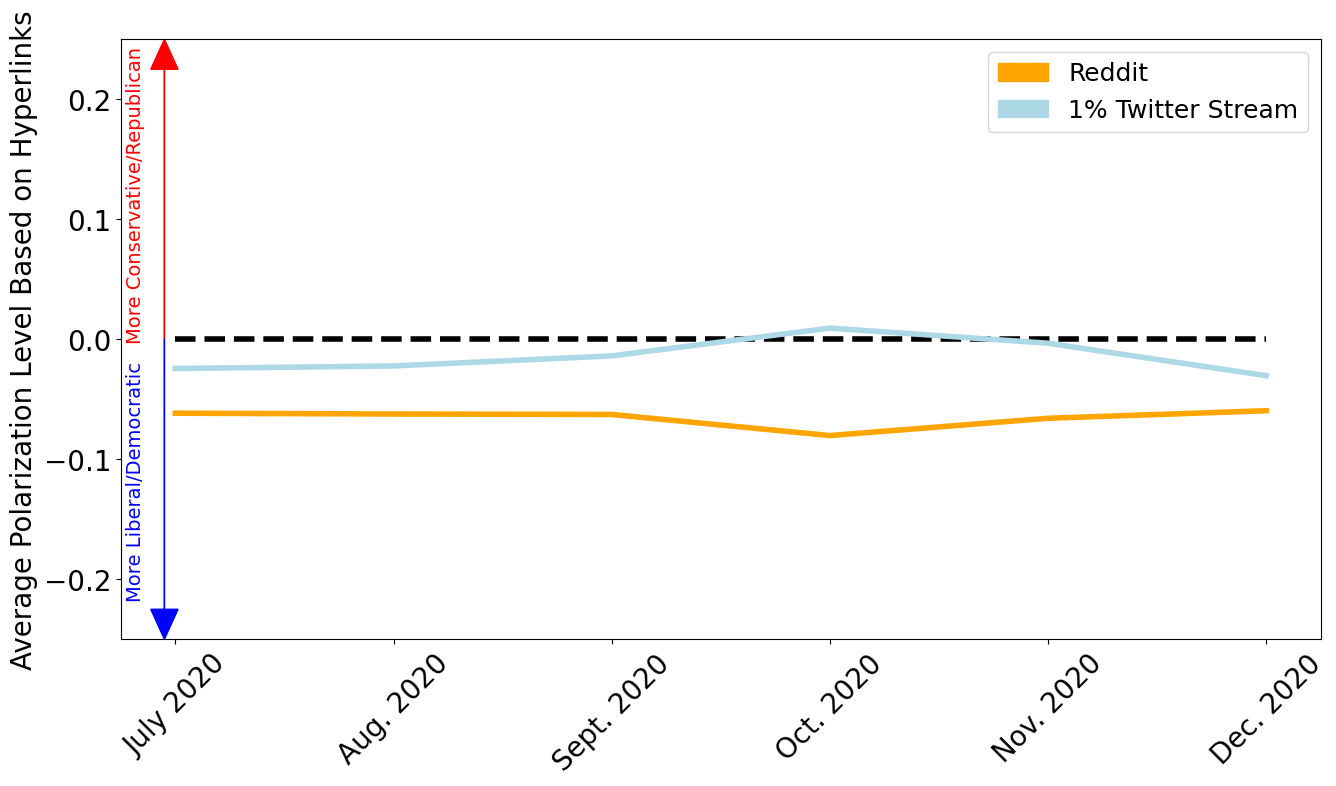
\includegraphics[width=1\linewidth]{figures/polarization_redidit_twitter.png}
\label{fig:cdf-subreddit-hyperlinks}
\end{subfigure}%
\begin{subfigure}{.48\textwidth}
  \centering
  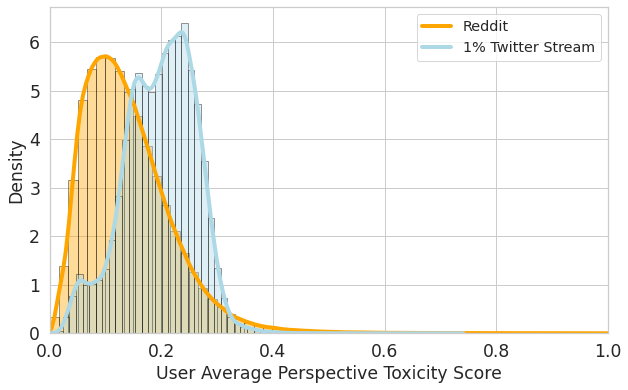
\includegraphics[width=1\linewidth]{figures/average-toxicity-distribution-end2020.png}
 \label{fig:cdf-user-hyperlinks}
\end{subfigure}
\label{fig:cdf-hyperlinsk}
\caption{\textbf{Relative Perspective toxicity of tweets and comments on Twitter and Reddit}--- Comparing a 1\% Twitter stream's Perspective API toxicity scores to the bulk of Reddit comments from  July to Decemebr 2020, we see that Reddit has maintained lower levels of toxicity over time and amongst users. }
\end{figure*}
As seen in Figures~\ref{}

Because of self-organizing and fairly norm-heavy communities form on Reddit, we find that our set of misinformation URLs are largely confined to a small set of subReddits and set of users. As seen in Figure~\ref{fig:cdf-subreddit-hyperlinks}, fairly few subReddits are responsible for the amount of Misinformation URLs Reddit Submissions. For instance, we find that only 133 Reddits were responsible for 90\% of Misinformation URL submission on Reddit from July 2020 to December 2020. Only 4007 contained misinformation URLS within their submissions. 4878 different subReddits contained misinformation URLs in their comments.While some of misinformation posts could have been removed by moderators and Reddit itself, this illustrates the moderating effect community norms have on the material that is posted and stays posted in  the majority of subreddits. This is largely in contrast to the number of subReddits containing authentic news URLs, with 513 subReddits containing 90\% of authentic news URL submissions and 12,825 containing authentic news Reddit Submissions. 18131 different subReddits had authentic news domain hyperlinks in their comments from July 2020 to December 2020. This behavior among subreddits largely caries over to the set of Reddit users who posted these links to misinformation and authentic news websites. As seen in Figure~\ref{fig:cdf-user-hyperlinks}, just 1423 users were responsible for 90.0\% of of misinformation URLs subReddit submissions in contrast to the 11,336 responsible for authentic news submissions. 
\begin{figure*}
\begin{subfigure}{.48\textwidth}
  \centering
  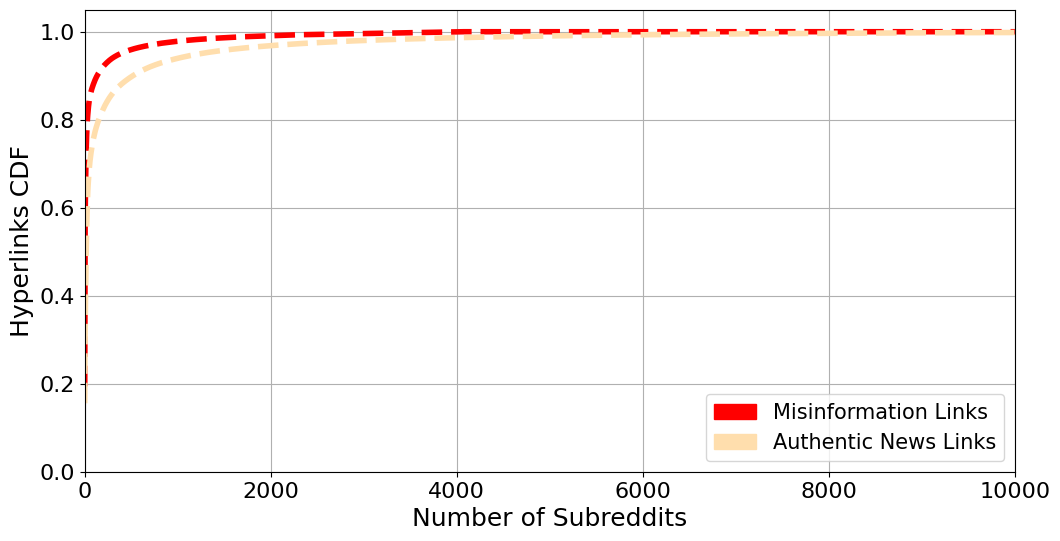
\includegraphics[width=1\linewidth]{figures/misinformation-authentic-cdf.png}
  \caption{\textbf{CDF News Hyperlinks by Subreddit}— Just 133 subreddits posted  90.0\% of hyperlinks to the misinformation websites in our dataset from July 2020 to December 2020. In contrast, 513 subReddits posted 90.0\% of the hyperlinks to authentic news websites during this same period. 
}
\label{fig:cdf-subreddit-hyperlinks}
\end{subfigure}%
\begin{subfigure}{.48\textwidth}
  \centering
  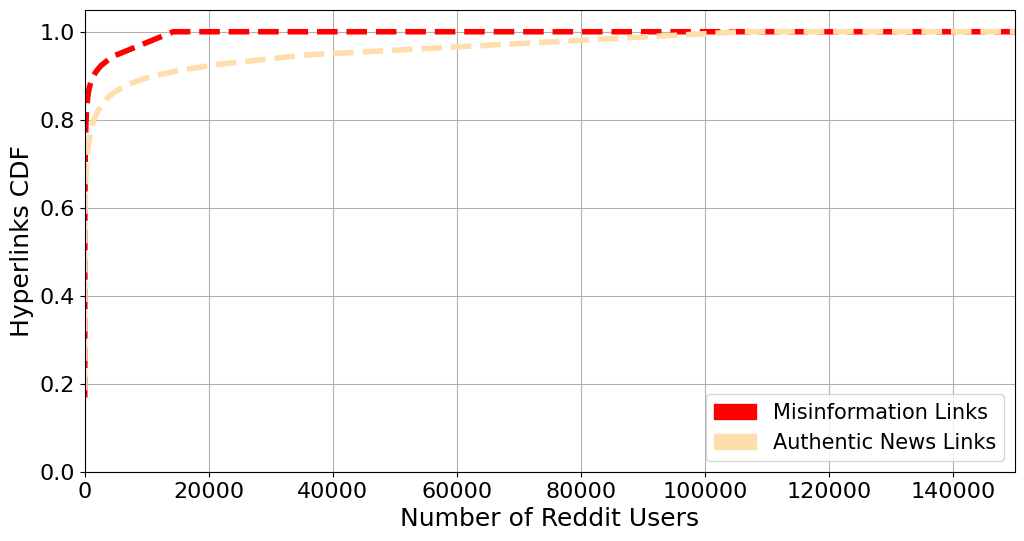
\includegraphics[width=1\linewidth]{figures/misinformation-authentic-users-cdf.png}
 \caption{\textbf{CDF News Hyperlinks by User}— Just 1423 subreddits posted  90.0\% of hyperlinks to the misinformation websites in our dataset from July 2020 to December 2020. In contrast, a whopping 11,336 subReddits posted 90.0\% of the hyperlinks to authentic news websites during this same period. 
}
 \label{fig:cdf-user-hyperlinks}
\end{subfigure}
\label{fig:cdf-hyperlinsk}
\end{figure*}


\begin{figure*}
\begin{subfigure}{.48\textwidth}
  \centering
  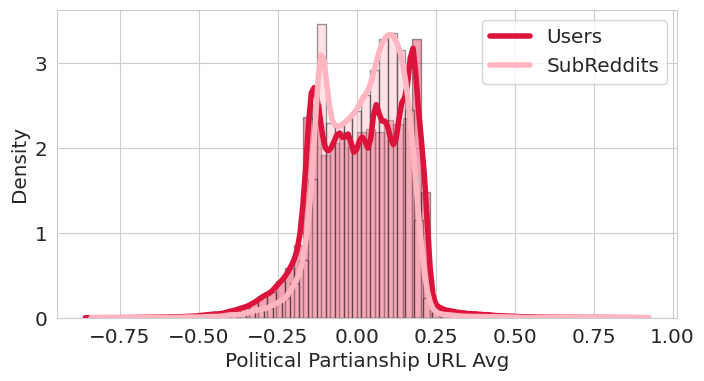
\includegraphics[width=1\linewidth]{figures/partisanship_avg.png}
 
\label{fig:partisanship-average}
\end{subfigure}%
\begin{subfigure}{.48\textwidth}
  \centering
  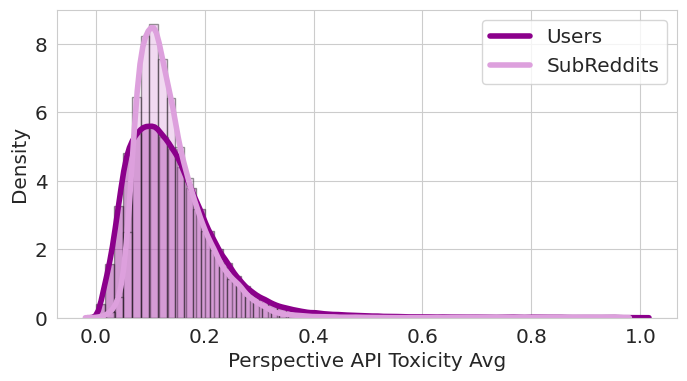
\includegraphics[width=1\linewidth]{figures/toxicity_avg.png}
 
 \label{fig:toxicity-average}
\end{subfigure}
\begin{subfigure}{.48\textwidth}
  \centering
  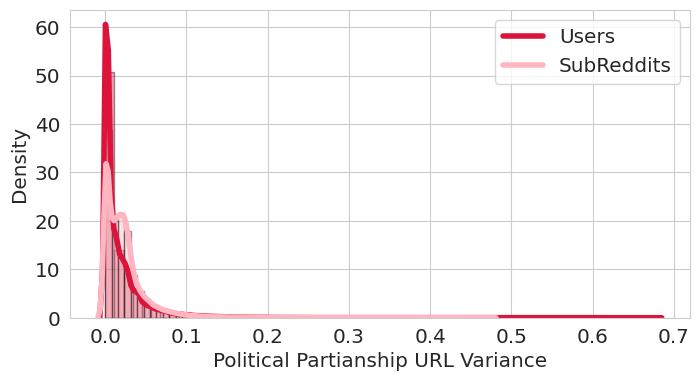
\includegraphics[width=1\linewidth]{figures/partisanship_variance.png}
 
\label{fig:partisanship-variance}
\end{subfigure}%
\begin{subfigure}{.48\textwidth}
  \centering
  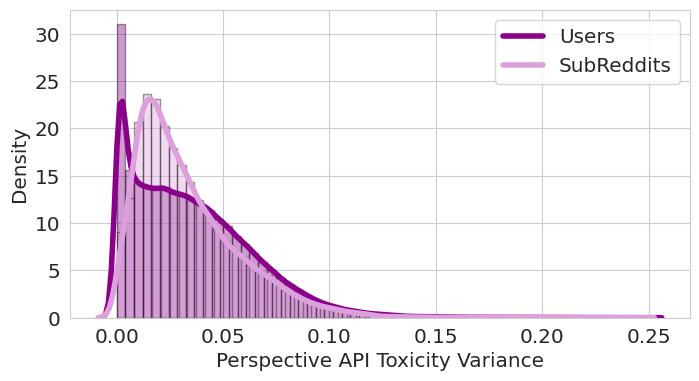
\includegraphics[width=1\linewidth]{figures/toxicity_variance.png}
 
 \label{fig:toxicity-variance}
\end{subfigure}
\caption{\textbf{Toxicity and Political URL Variation among Users and SubReddits }--- As seen above, there are relatively tight windows of political partisanship and toxicity among subreddits with subreddits having approximately little more diversity than individual users. 
}
\label{fig:diversity-of-views}
\end{figure*}
\begin{figure*}
\begin{subfigure}{.48\textwidth}
  \centering
  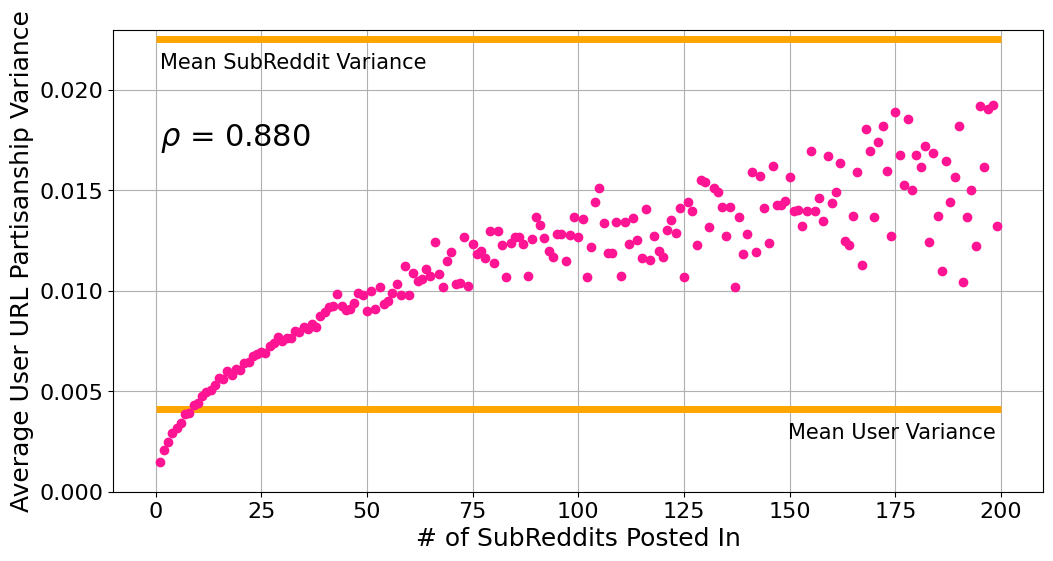
\includegraphics[width=1\linewidth]{figures/numberOfSubRedditsByPartianshipAvg.png}
  \caption{\textbf{User SubReddit Paritipation vs Variance in Political URLs Posted}-
}
\label{fig:participation-political}
\end{subfigure}%
\begin{subfigure}{.48\textwidth}
  \centering
  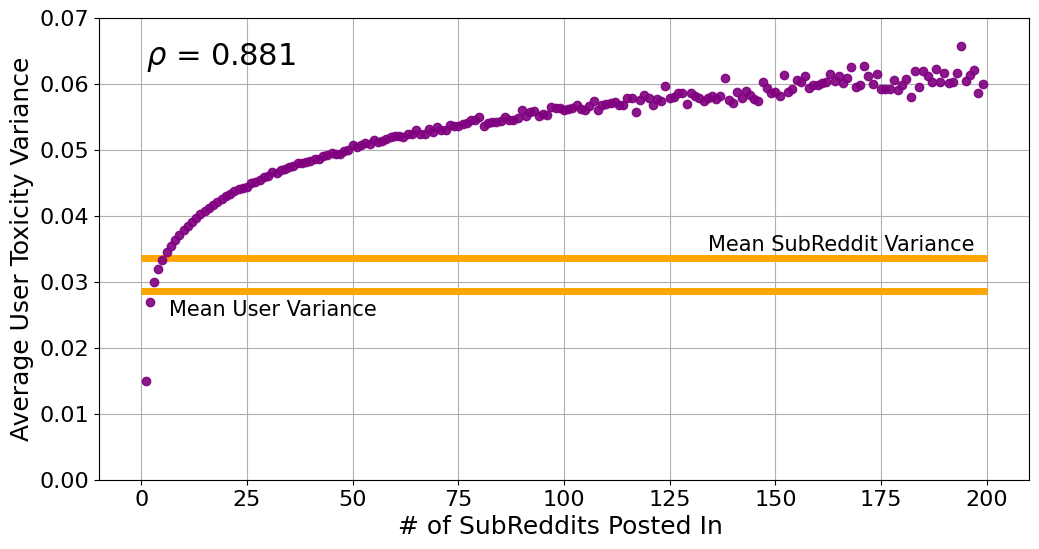
\includegraphics[width=1\linewidth]{figures/numberOfSubRedditsByToxicityAvg.png}
 \caption{\textbf{User SubReddit Paritipation vs Variance in Comment Toxicity}— 
}
 \label{fig:participation-toxicity}
\end{subfigure}
\caption{\textbf{Relative amounts of partisanship and toxicity diversity among individual users by SubReddit participation }--- As users participate in more and more the variance of their behavior increases with user posting a wider variety of political websites and commenting with a wider berth of toxicity. 
}
\label{fig:participation}
\end{figure*}
The moderating effect of subReddits is further seen in the relatively narrow window of political views and level of toxicity that are allowed within each subReddit community. As seen in Figure~\ref{fig:diversity-of-views}, there relatively narrow windows of allowed divergence in political beliefs and toxicity among SubRedits and users. This is in Figure~\ref{fig:participation}, as only as users participate in more and more subReddits does the berth of different types of comments that they post increase. On average, after a user participates in TODO subreddits the variance of their toxicity exceeds the average subReddit (an entire community). This illustrates the ability of subReddit communities to maintain an equilibrium of acceptable toxicity on their platforms, excising redditors who go outside normal bounds as illutrated in prior work~\cite{rajadesingan2020quick}.  Similarly, we find  that as users participate and post in more subReddits, they post a wider political range of websites.


\begin{figure*}
\begin{subfigure}{.48\textwidth}
  \centering
  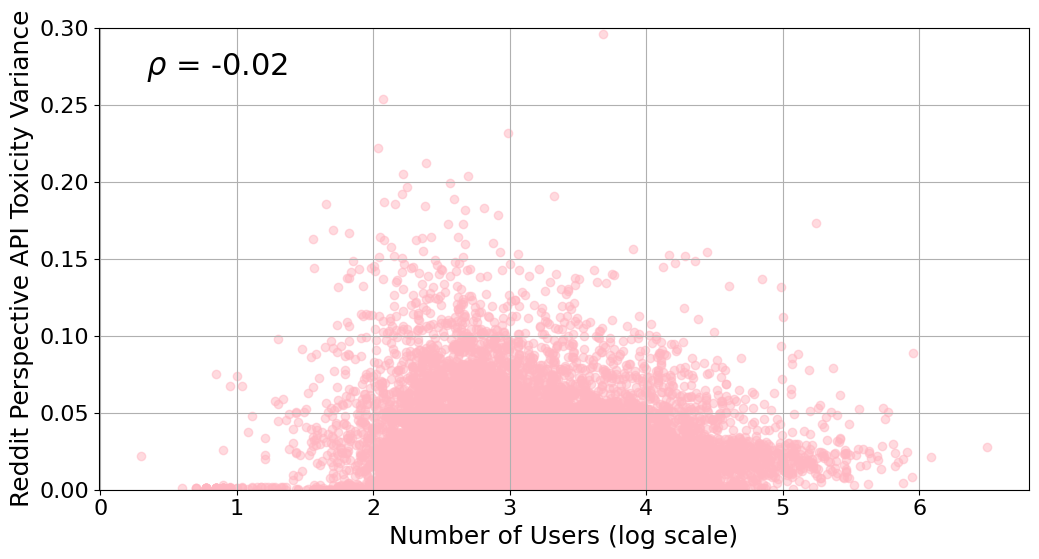
\includegraphics[width=1\linewidth]{figures/user-partisanship-var.png}
  \caption{\textbf{Number of SubReddit Users vs Variance in Political URLs Posted}-
}
\label{fig:participation-political}
\end{subfigure}%
\begin{subfigure}{.48\textwidth}
  \centering
  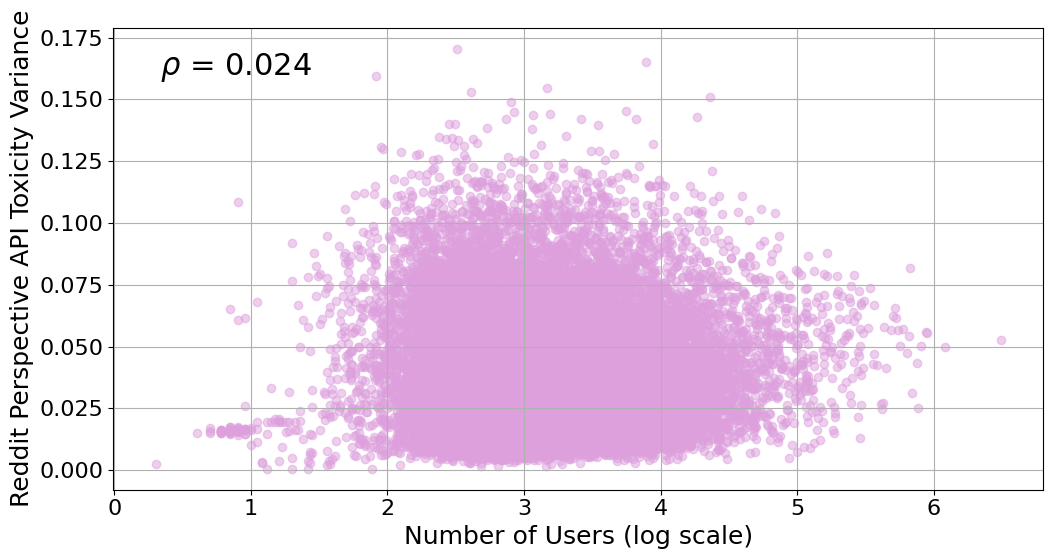
\includegraphics[width=1\linewidth]{figures/user-toxicity-var.png}
 \caption{\textbf{Number of SubReddit Users vs Variance in Comment Toxicity}— 
}
 \label{fig:participation-toxicity}
\end{subfigure}
\begin{subfigure}{.48\textwidth}
  \centering
  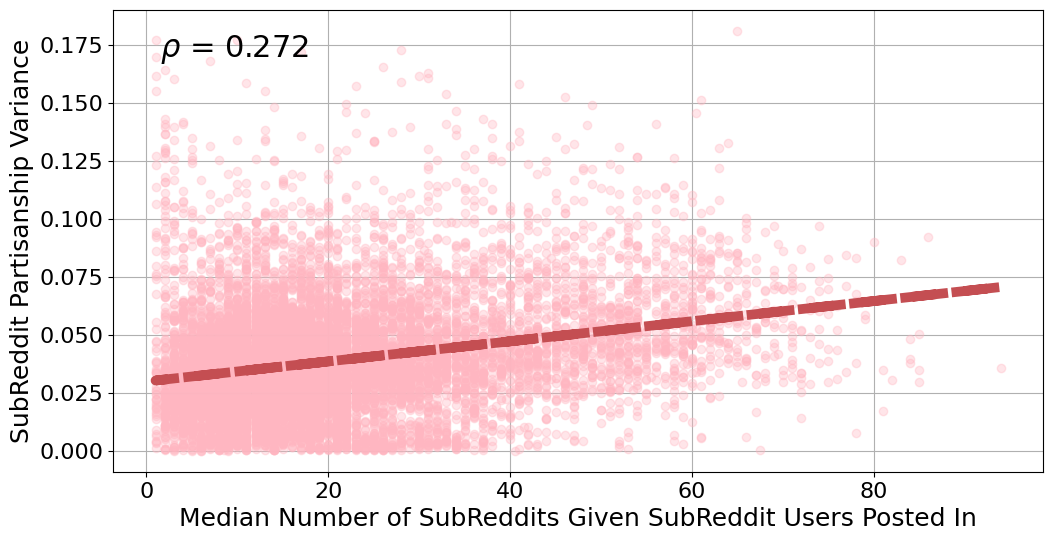
\includegraphics[width=1\linewidth]{figures/partisanship-to-num-subreddits.png}
 
\label{fig:particiption-median-toxicity}
\end{subfigure}%
\begin{subfigure}{.48\textwidth}
  \centering
  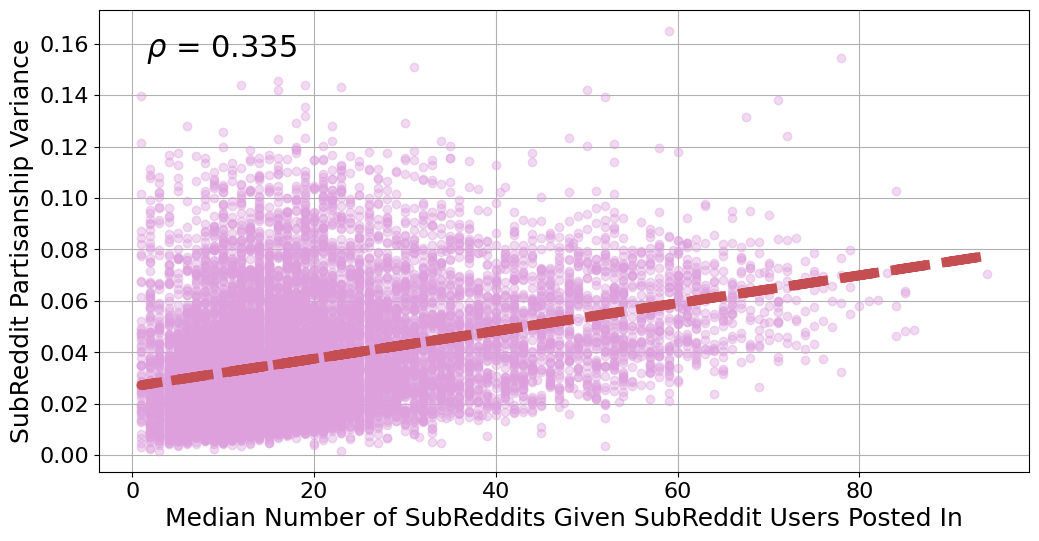
\includegraphics[width=1\linewidth]{figures/toxicity-to-num-subreddits.png}

 \label{fig:cdf-user-hyperlinks}
\end{subfigure}
\label{fig:cdf-hyperlinsk}
\caption{\textbf{Number of Users to Variance in SubReddit Behavior}--- As the number of users in a particular subReddit increases, there is no discernible trend in the the variance of political URLS posted nor the Perspective API toxicity. However, as the the number of subReddits that the median user participates in increases within a given subReddit, the variance in political URLs and the the variance in toxicity does increase.  
}
\label{fig:participation}
\end{figure*}

Conversely, we find that the number of users that a subReddit contains, does not correlate with the diversity of toxicity and political views present on that subReddit. As seen in Figure~\ref{fig:participation}, as the number of users that post submissions in a subReddit increases, there is no discernible correlation with the variance of toxicity nor the variance of political views voiced on that subReddit. In contrast, we find that as the median subReddit participation on Reddit increases, the variance of toxicity and political viewd does increase.  Namely, if a subReddit has users that participate in a wide range of subReddits outside that particular subReddit, then this particular subReddit has higher levels of variance in political views and toxicity. This suggests that amount of people that a subReddit does not correspond with diversity of views and behavior on that subReddit but rather with the amount of communities that that subReddit's users come from and with which they engages. 
\begin{figure*}
\begin{subfigure}{.48\textwidth}
  \centering
  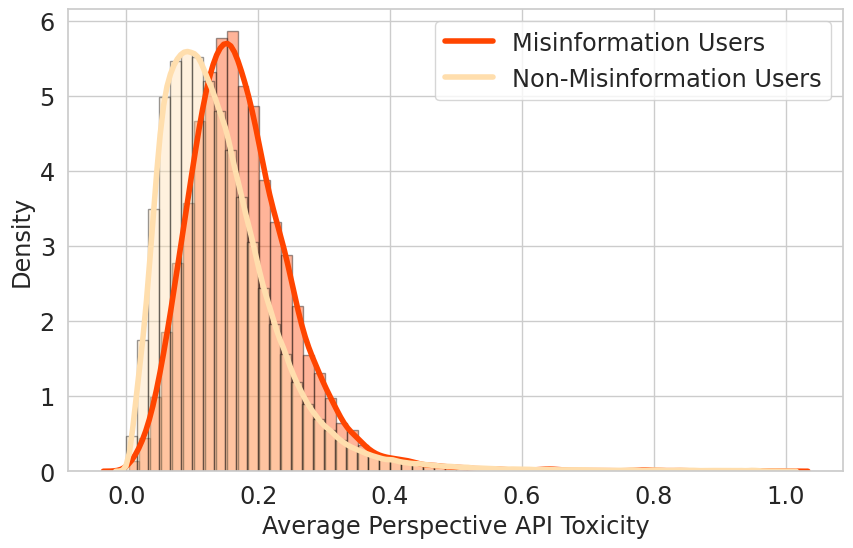
\includegraphics[width=1\linewidth]{figures/user-misinfo-toxicity.png}
\label{fig:user-misnformation}
\end{subfigure}%
\begin{subfigure}{.48\textwidth}
  \centering
  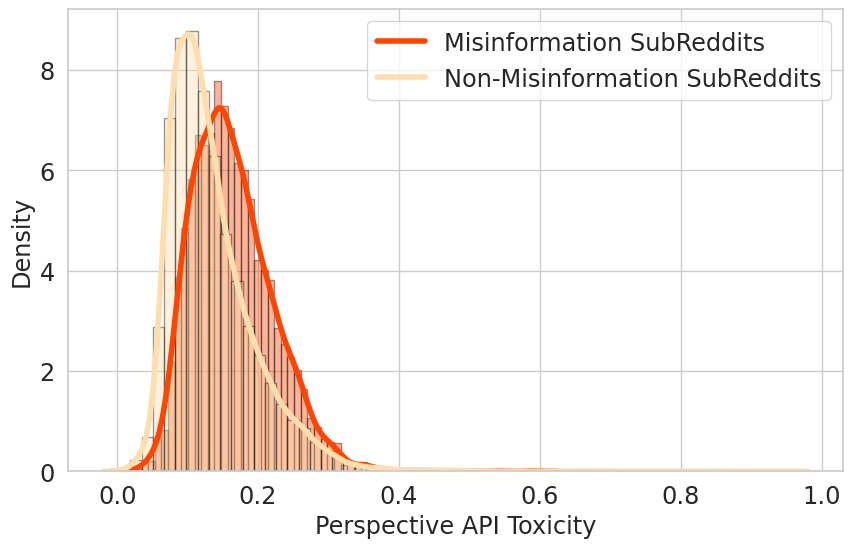
\includegraphics[width=1\linewidth]{figures/reddit-misinfo-toxicity.png}
 \label{fig:reddit-misinformation}
\end{subfigure}
\label{fig:misinformation-reddit-user}
\end{figure*}
Having established how the characteristics of subReddits exerts norms over their particular users, we now turn to understand how these norms affect the levels of misinformation on Reddit platform and on particular subReddits. 
As seen in Figure~\ref{fig:misinformation-reddit-user}, as on Twitter, misinformation subReddits as well as have higher levels of toxicity compared with subReddis with not misinformatino submissions. 

Looking a





